% paquetes, configuración, y título
\documentclass[journal,twoside]{IEEEtran}

\usepackage[utf8]{inputenc}
\usepackage[spanish, es-tabla]{babel}
\usepackage{amssymb, amsmath, amsthm , amsfonts}
\usepackage{graphicx, float, subcaption}
\usepackage{siunitx}
\usepackage{enumerate}
\usepackage{listings}
\usepackage{booktabs}
\usepackage{fancyhdr}
\usepackage{multirow}
\usepackage{tabularx}
\usepackage{colortbl}
\usepackage{array}
\usepackage[export]{adjustbox}
\usepackage[usenames,dvipsnames]{color}
\usepackage{cite}
%Usar \url{http...} para links
\usepackage{url}
%O también \href{http...}{text}
\usepackage{hyperref}
%Con \gamma sale cursiva, \upgamma sale recta
\usepackage{upgreek}
%Usar $ 220\phase{3\degree} $
\usepackage{steinmetz}
%Usar \degree para sacar un °
\usepackage{gensymb}
%Negrilla para formulas $ \bm{x} $
\usepackage{bm}
% Se puede usar $ \sfrac{x}{y} $
\usepackage{xfrac}
%pueden ingresar imagenes en .eps
\usepackage{epstopdf}
\usepackage{float}
%\graphicspath{ {images/} }
\setlength{\parskip}{\baselineskip}
\raggedbottom
%Cambia nombre default de table
%\AtBeginDocument{%
%\renewcommand{\tablename}{TABLA}}
%Cambia nombre default de keywords
%\renewcommand{\IEEEkeywords}{\small\textsl{\textbf{Palabras claves---}}}
%Cambia nombre default de figuras
%\renewcommand{\figurename}{Figura}
%Cambia nombre default de referencias
%\renewcommand{\refname}{Referencias}
%Pueden usar $ \abs{x} $ para |x| 
\providecommand{\abs}[1]{\lvert#1\rvert}

\decimalpoint

\title{
    Informe de Laboratorio No.~ 1 \\
    Efecto de Carga en Instrumentos de Medición \\
    Electrónica Análoga II - 2016496
}


\author{
    \IEEEauthorblockN{
        Juan Sebastian Alba Narvaez, 
        Jorge Luis Ladeus Machado, 
        David Alejandro Riano Sarmiento \\
        \{jalban, jladeus, darianos\}@unal.edu.co}\\
    \IEEEauthorblockA{
        Departamento de Ingeniería Eléctrica y Electrónica\\
        Universidad Nacional de Colombia. Bogotá D.C., Colombia.\\
    }
}
\renewcommand{\leftmark}{Laboratorio de Electrónica Análoga II - 2024-1} 

\begin{document}
\maketitle

\renewcommand{\abstract}{\small\textsl{\textbf{Abstract---}}}
\renewcommand{\IEEEkeywords}{\small\textsl{\textbf{Palabras claves---}}} 
\begin{abstract}
The effects of load are explored for measurement instruments, particularly in the case of Analog 2 devices. Significant load and measurement precision relationships are determined. The study emphasizes the importance of taking loads into account when calibrating instruments, as well as when interpreting data. Insights are provided which may enhance the reliability of instruments in practical settings.
\end{abstract}

\begin{IEEEkeywords}
Efecto de carga, instrumentos de medición, respuesta en frecuencia.
\end{IEEEkeywords}

\section{Introducción}
En la practica de circuitos la realización de mediciones es una tarea bastante común y
que se realiza cotidianamente para poder observar el funcionamiento real de un
circuito en comparación con el funcionamiento teórico esperado e identificar si está o no 
funcionando de manera correcta.
Para un buen ejercicio de medición se requieren instrumentos adecuados para la medición
y habilidad para operar e interpretar los resultados del dispositivo.
Dichas habilidades incluyen el reconocer factores prácticos del funcionamiento de estos
que afectan las mediciones, y que deben ser tenidas en cuenta al determinar si un 
instrumento es adecuado para realizar una medición en un circuito con características
dadas. Uno de estos aspectos prácticos es el efecto de carga.
Para explorar las implicaciones de este fenómeno al realizar mediciones
en circuitos a baja y alta frecuencia, se propone realizar mediciones de tensión 
con un osciloscopio y un multímetro en un circuito resistivo, utilizando
un generador de señales para producir señales de frecuencia variable y así observar
también la respuesta en frecuencia asociada a la presencia de impedancias reactivas
en los instrumentos, que a su vez afectan el efecto de carga.


\section{Marco Teórico}

\subsection{Efecto de carga}
Este se refiere a la modificación (indeseada) de las señales
de entrada o de salida de dispositivos electrónicos debido a la presencia de una 
resistencia de entrada o de salida, respectivamente. Este es un factor importante
a tener encuentra en los instrumentos de laboratorio debido a la necesidad de 
resultados precisos.

Para un dispositivo de medición de tensión conectado en paralelo a una carga a 
través de la cual para una corriente, sobre la cual se va a realizar la medición, 
como se muestra en Fig.~\ref{fig:vmeas}e tiene que la medición de entrada, 
$V_i$, al dispositivo será

\begin{figure}[H]
    \centering
    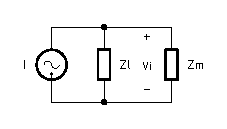
\includegraphics[width=\columnwidth]{img/circ/vmeas.pdf}
    \caption{Dispositivo midiendo tensión \\en paralelo a carga.}
    \label{fig:vmeas}
\end{figure}
\vspace{-20pt}
\begin{align*}
    V_i &= I(Z_l || Z_m) \\
    \lim_{Z_m\to\inf} V_i &= IZ_l
    \label{Ecucaion de paralelo con Zm inf}
\end{align*}


Es decir, la impedancia de entrada del voltímetro genera una disminución en la
tensión entre las terminales de la medición, siendo necesario una impedancia
muy alta para evitar alterar el circuito original y obtener una medición más 
precisa.

Para el caso de un dispositivo de generación de tensión, la tensión de salida 
$V_o$ que efectivamente se provee al circuito al cual está conectado,
Fig.~ \ref{fig:vmeas}, será

\begin{figure}[H]
    \centering
    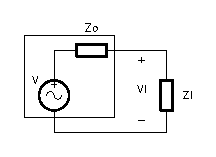
\includegraphics[width=\columnwidth]{img/circ/vsource.pdf}
    \caption{Generador de tensión/señales.}
    \label{fig:vsource}
\end{figure}

\begin{equation}
    \begin{split}
        V_o &= V\frac{R_l}{R_l + R_o} \\
    \lim_{Z_o\to 0} V_o &= V_o
    \label{2}
    \end{split}
\end{equation}


Debido a lo cual en los dispositivos de generación de tensión como fuentes de 
tensión y generadores de señales se busca que la resistencia de salida del dispositivo sea lo menor posible para lograr que la tensión generada por el 
dispositivo se transmita de manera adecuada a la carga.

\subsection{Respuesta en frecuencia y ancho de banda}
El anterior análisis para estado estable hace uso de impedancias
en vez  de resistencias, pues algunos dispositivos suelen tener
un componente reactivo de entrada o salida, las cuales causan que estos
tengan un cambio de magnitud a lo largo de grandes rangos de frecuencia, 
funcionando efectivamente como filtros pasa-banda o pasa-baja. Esto significa
que los instrumentos sólo funcionan de manera adecuada dentro de un rango
de frecuencias en las cuales la impedancia reactiva es lo suficientemente grande
o pequeña para que sus efectos puedan ser ignorados. A este rango se le llama ancho de banda.

Aunque las impedancias de entrada y salida están involucradas en el ancho de
banda de un instrumento, también la respuesta a frecuencia en componentes
internos es un factor importante que está involucrado, por lo que es posible que
un dispositivo pueda no funcionar dentro del rango definido por las impedancias
de entrada o salida debido a que está limitado por un menor rango definido por
los componentes internos.



\section{Procedimiento}
Se van a realizar mediciones de tensión con un osciloscopio y un multímetro en
un circuito con varias cargas pasivas y observar el efecto de carga que efectúan
las impedancias de los instrumentos sobre las mediciones, utilizando una fuente
sinusoidal a lo lago de un rango de bajas y altas frecuencias.

Para esto se van a utilizar las siguientes circuitos que modelan la impedancia
de entrada de un osciloscopio junto con las sondas de medición  (Fig.~\ref{fig:oscilloscope-probes}), y un voltímetro (Fig.~\ref{fig:voltmeter}).
Tanto el voltímetro como el osciloscopio y las sondas se representan como 
resistencias en paralelo con capacitores. 

\begin{figure}[H]
    \centering
    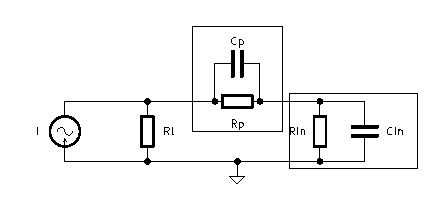
\includegraphics[width=\columnwidth]{img/circ/oscilloscope-probes.pdf}
    \caption{Modelo de la impedancia del osciloscopio y las sondas.}
    \label{fig:oscilloscope-probes}
\end{figure}
La tensión de entrada en el osciloscopio se puede expresar en función de la 
frecuencia cómo
\[
    H(s) = \frac{V(s)}{I(s)} = \frac{R_l R_{in}}{R_p + R_{in} + R_l}
        \frac{s\left(\frac{1}{C_p R_p}\right)^{-1} + 1 }
            {s \left(\frac{R_p + R_{in} + R_l}{C_{in} R_{in} R_p + C_p R_p R_{in}}\right)^{-1} + 1}
\]

Se muestra la presencia de un cero simple seguido por un polo, indicando
un comportamiento de filtro pasa-banda.

\begin{figure}[H]
    \centering
    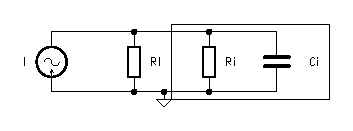
\includegraphics[width=\columnwidth]{img/circ/voltmeter.pdf}
    \caption{Modelo de la impedancia de entrada de un multímetro.}
    \label{fig:voltmeter}
\end{figure}

En el caso del multímetro, 
\[
    H(s) = \frac{V(s)}{I(s)} = \frac{R_i}{R_i + R_l} \frac{1}
        {1 + s\left(\frac{R_i + R_l}{C_i R_i R_l}\right)^{-1}}
\]

en donde se puede observar sólo un polo, sin ceros, característico del 
comportamiento de un filtro pasa-bajas. 

\subsection{Simulación}

\begin{table*}[!ht]
    \centering
    \begin{tabular}{|l|l|l|l|}
    \hline
        Nombre & Ancho de banda & $Z_{in}$ & $Z_{out}$ \\ \hline
        Osciloscopio USB OWON VDS1022I & $25\si{\mega\hertz}$ & $1\si{\mega\hertz}+2\%$ paralelo con $15\si{\pico\farad}  \pm 5\si{\pico\farad}$ & - \\ \hline
        Generador de señales ICL8038 & 0.001Hz - 400 kHz & - & $200\si{\ohm}$ \\ \hline
        Multimetro OWON Digital Bluetooth & 10 MHz & $10\si{\mega\ohm}$ paralelo con  10 pF$^{*}$& - \\ \hline
        Sondas P6060 & 40 MHz & $1\si{\mega\ohm}$ paralelo con 95 pF & - \\ \hline
    \end{tabular}
    \caption{Impedancias de entrada y salida de los instrumentos usados. *Se asume un valor común, pues la capacitancia de entrada no estaba especificada en la hoja de datos.}
    \label{tab:instruments-specs}
\end{table*}

La comprobación de estas observaciones
puede ser realizada por medio del gráfico de Bode de los respectivos circuitos,
los cuales pueden ser obtenidos por medio de programas de simulación de circuitos.
Se especifican los circuitos en el software LTSpice usando resistencias de carga
de $R_l = 10\si{\kilo\ohm}$, y los valores nominales de las impedancias
de los instrumentos con los que se va a trabajar, mostrados en la Tabla 
\ref{tab:instruments-specs}.
Se usa una fuente de corriente sinusoidal de amplitud $1\si{\ampere}$, con un
barrido de frecuencias de $0.1\si{\hertz}$ a $10\si{\mega\hertz}$ y se obtienen
las gráficas de Bode de la tensión de entrada en el osciloscopio y el multímetro.


\section{Resultados y Análisis}

\begin{figure}[!h]
    \centering
    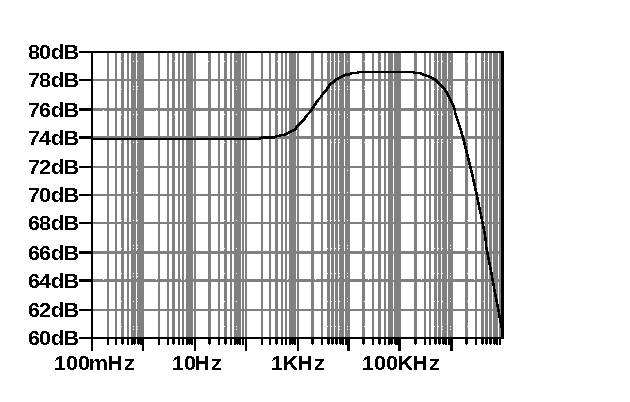
\includegraphics[width=\columnwidth]{img/graphs/oscilloscope-probes-model-bode.pdf}
    \caption{Diagrama de Bode del modelo del osciloscopio y las sondas de medición.}
    \label{fig:oscilloscope-probes-model-bode}
\end{figure}
\begin{figure}[!h]
    \centering
    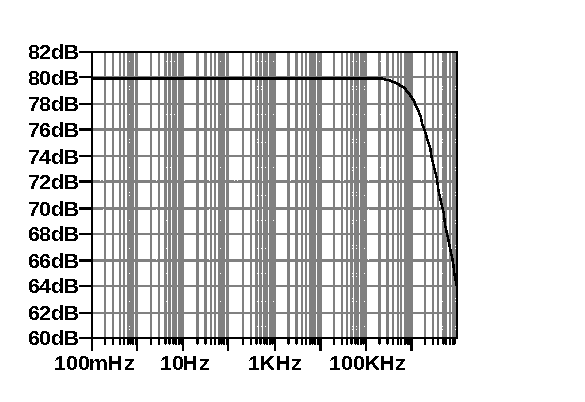
\includegraphics[width=\columnwidth]{img/graphs/voltmeter-model-bode.pdf}
    \caption{Diagrama de Bode del modelo del multímetro.}
    \label{fig:voltmeter-model-bode}
\end{figure}

Se puede observar en la forma de las gráficas que efectivamente
la impedancia reactiva de las sondas y el osciloscopio causa que a 
altas frecuencias estos se comporten cono un filtro pasa-banda con 
frecuencia de corte aproximadas inferior de $10\si{\kilo\hertz}$ y 
superior de $500\si{\kilo\hertz}$. Mientras que el multímetro aparece
como un filtro basa-bajas con frecuencia de corte de alrededor de
$500\si{\kilo\hertz}$.


\subsection{Implementación}
Para la observación de el efecto de carga a se utilizara el siguiente circuito:

\begin{figure}[H]
    \centering
    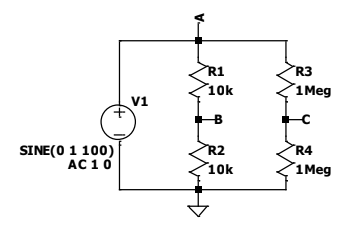
\includegraphics[scale=0.65]{img/circ/Circuito para efecto de carga.png}
    \caption{Circuito de efecto de carga}
    \label{Circuito de efecto de carga}
\end{figure}

Para empezar tomaremos medidas de voltaje con multímetro y osciloscopio para 1Vp y 100Hz para ver las mediciones que los equipos proporcionan
\\
\\
Multímetro:
\begin{table}[H]
\centering
\begin{tabular}{l|cll|}
\cline{2-4}
                          & \multicolumn{3}{c|}{Voltaje (mV)}                                  \\ \hline
\multicolumn{1}{|l|}{Hz}  & \multicolumn{1}{c|}{Nodo A} & \multicolumn{1}{l|}{Nodo B} & Nodo C \\ \hline
\multicolumn{1}{|l|}{100} & \multicolumn{1}{l|}{702.5}  & \multicolumn{1}{l|}{307.5}  & 320.3  \\ \hline
\end{tabular}
\end{table}
Osciloscopio:

\begin{figure}[H]
    \centering
    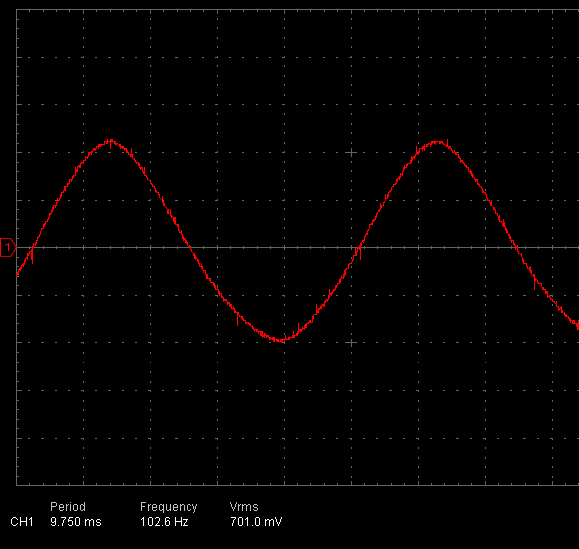
\includegraphics[scale=0.5]{img/Osci/Nodo A 100Hz.png}
    \caption{Nodo A}
    \label{Nodo A}
\end{figure}

\begin{figure}[H]
    \centering
    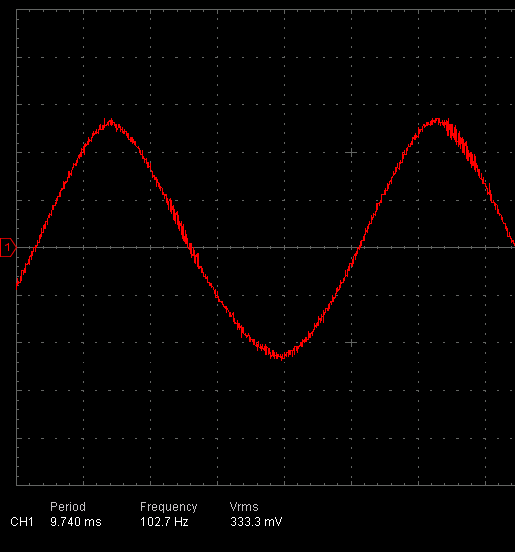
\includegraphics[scale=0.5]{img/Osci/Nodo B 100Hz.png}
    \caption{Nodo B}
    \label{Nodo B}
\end{figure}

\begin{figure}[H]
    \centering
    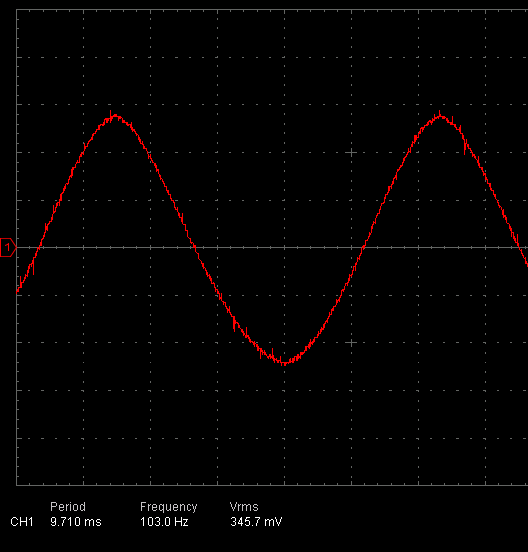
\includegraphics[scale=0.5]{img/Osci/Nodo C 100Hz.png}
    \caption{Nodo C}
    \label{Nodo C}
\end{figure}

Ahora veremos como a diferentes frecuencias se ven afectadas las mediciones por cambios en la frecuencia del generador de señal que tiene 4 rangos de frecuencias; midiendo en los distintos nodos mostrados en la figura \ref{Circuito de efecto de carga}:\\

Rango de 5Hz a 50 Hz:

\begin{table}[H]
\centering
\begin{tabular}{l|lll|}
\cline{2-4}
                         & \multicolumn{3}{c|}{Voltaje (mV)}                                  \\ \hline
\multicolumn{1}{|l|}{Hz} & \multicolumn{1}{c|}{Nodo A} & \multicolumn{1}{l|}{Nodo B} & Nodo C \\ \hline
\multicolumn{1}{|l|}{5}  & \multicolumn{1}{l|}{629.6}  & \multicolumn{1}{l|}{300.5}  & 312.7  \\ \hline
\multicolumn{1}{|l|}{10} & \multicolumn{1}{l|}{634.6}  & \multicolumn{1}{l|}{302.8}  & 315.4  \\ \hline
\multicolumn{1}{|l|}{15} & \multicolumn{1}{l|}{641.8}  & \multicolumn{1}{l|}{302.8}  & 315.5  \\ \hline
\multicolumn{1}{|l|}{20} & \multicolumn{1}{l|}{638.1}  & \multicolumn{1}{l|}{304.7}  & 319.6  \\ \hline
\multicolumn{1}{|l|}{25} & \multicolumn{1}{l|}{642.4}  & \multicolumn{1}{l|}{303.5}  & 318.4  \\ \hline
\multicolumn{1}{|l|}{30} & \multicolumn{1}{l|}{643.3}  & \multicolumn{1}{l|}{304.4}  & 319.7  \\ \hline
\multicolumn{1}{|l|}{35} & \multicolumn{1}{l|}{642.5}  & \multicolumn{1}{l|}{302.7}  & 317.7  \\ \hline
\multicolumn{1}{|l|}{40} & \multicolumn{1}{l|}{643.5}  & \multicolumn{1}{l|}{305.1}  & 319.3  \\ \hline
\multicolumn{1}{|l|}{45} & \multicolumn{1}{l|}{643.4}  & \multicolumn{1}{l|}{305.4}  & 319.9  \\ \hline
\multicolumn{1}{|l|}{50} & \multicolumn{1}{l|}{641.6}  & \multicolumn{1}{l|}{304.7}  & 319.3  \\ \hline
\end{tabular}
\end{table}

Rango de 50Hz a 500Hz:

\begin{table}[H]
\centering
\begin{tabular}{l|lll|}
\cline{2-4}
                          & \multicolumn{3}{c|}{Voltaje (mV)}                                  \\ \hline
\multicolumn{1}{|l|}{Hz}  & \multicolumn{1}{c|}{Nodo A} & \multicolumn{1}{l|}{Nodo B} & Nodo C \\ \hline
\multicolumn{1}{|l|}{50} & \multicolumn{1}{l|}{641.6}  & \multicolumn{1}{l|}{304.7}  & 319.3  \\ \hline
\multicolumn{1}{|l|}{100} & \multicolumn{1}{l|}{648.5}  & \multicolumn{1}{l|}{305.8}  & 321.5  \\ \hline
\multicolumn{1}{|l|}{150} & \multicolumn{1}{l|}{639.5}  & \multicolumn{1}{l|}{306.1}  & 320.2  \\ \hline
\multicolumn{1}{|l|}{200} & \multicolumn{1}{l|}{644.6}  & \multicolumn{1}{l|}{306.7}  & 322.1  \\ \hline
\multicolumn{1}{|l|}{250} & \multicolumn{1}{l|}{649.7}  & \multicolumn{1}{l|}{305.8}  & 321.2  \\ \hline
\multicolumn{1}{|l|}{300} & \multicolumn{1}{l|}{645.9}  & \multicolumn{1}{l|}{306.5}  & 320.8  \\ \hline
\multicolumn{1}{|l|}{350} & \multicolumn{1}{l|}{643.8}  & \multicolumn{1}{l|}{305.7}  & 321    \\ \hline
\multicolumn{1}{|l|}{400} & \multicolumn{1}{l|}{646.4}  & \multicolumn{1}{l|}{306.1}  & 321.6  \\ \hline
\multicolumn{1}{|l|}{450} & \multicolumn{1}{l|}{648.6}  & \multicolumn{1}{l|}{306.7}  & 322.1  \\ \hline
\multicolumn{1}{|l|}{500} & \multicolumn{1}{l|}{647.8}  & \multicolumn{1}{l|}{306.5}  & 321.2  \\ \hline
\end{tabular}
\end{table}

Rango de 500Hz a 20kHz:

\begin{table}[H]
\centering
\begin{tabular}{l|lll|}
\cline{2-4}
                            & \multicolumn{3}{c|}{Voltaje (mV)}                                  \\ \hline
\multicolumn{1}{|l|}{Hz}    & \multicolumn{1}{c|}{Nodo A} & \multicolumn{1}{l|}{Nodo B} & Nodo C \\ \hline
\multicolumn{1}{|l|}{500} & \multicolumn{1}{l|}{647.8}  & \multicolumn{1}{l|}{306.5}  & 321.2  \\ \hline
\multicolumn{1}{|l|}{1000}  & \multicolumn{1}{l|}{649.5}  & \multicolumn{1}{l|}{307.6}  & 323.2  \\ \hline
\multicolumn{1}{|l|}{2000}  & \multicolumn{1}{l|}{659.4}  & \multicolumn{1}{l|}{309.7}  & 328.9  \\ \hline
\multicolumn{1}{|l|}{3000}  & \multicolumn{1}{l|}{664.5}  & \multicolumn{1}{l|}{307.7}  & 331.2  \\ \hline
\multicolumn{1}{|l|}{4000}  & \multicolumn{1}{l|}{668.7}  & \multicolumn{1}{l|}{306.8}  & 333.8  \\ \hline
\multicolumn{1}{|l|}{5000}  & \multicolumn{1}{l|}{670.6}  & \multicolumn{1}{l|}{303.5}  & 334.1  \\ \hline
\multicolumn{1}{|l|}{6000}  & \multicolumn{1}{l|}{675.2}  & \multicolumn{1}{l|}{299.7}  & 335.4  \\ \hline
\multicolumn{1}{|l|}{7000}  & \multicolumn{1}{l|}{675.5}  & \multicolumn{1}{l|}{293.4}  & 336.2  \\ \hline
\multicolumn{1}{|l|}{8000}  & \multicolumn{1}{l|}{676.7}  & \multicolumn{1}{l|}{290.1}  & 337.8  \\ \hline
\multicolumn{1}{|l|}{9000}  & \multicolumn{1}{l|}{678.2}  & \multicolumn{1}{l|}{281.4}  & 338.1  \\ \hline
\multicolumn{1}{|l|}{10000} & \multicolumn{1}{l|}{678.4}  & \multicolumn{1}{l|}{277.5}  & 338.2  \\ \hline
\multicolumn{1}{|l|}{11000} & \multicolumn{1}{l|}{679.2}  & \multicolumn{1}{l|}{270.4}  & 339.2  \\ \hline
\multicolumn{1}{|l|}{12000} & \multicolumn{1}{l|}{678.5}  & \multicolumn{1}{l|}{269.2}  & 339.8  \\ \hline
\multicolumn{1}{|l|}{13000} & \multicolumn{1}{l|}{680.2}  & \multicolumn{1}{l|}{254.5}  & 340.8  \\ \hline
\multicolumn{1}{|l|}{14000} & \multicolumn{1}{l|}{681.7}  & \multicolumn{1}{l|}{252.3}  & 341.1  \\ \hline
\multicolumn{1}{|l|}{15000} & \multicolumn{1}{l|}{682.7}  & \multicolumn{1}{l|}{242.8}  & 342.6  \\ \hline
\multicolumn{1}{|l|}{16000} & \multicolumn{1}{l|}{683.4}  & \multicolumn{1}{l|}{237.3}  & 343.5  \\ \hline
\multicolumn{1}{|l|}{17000} & \multicolumn{1}{l|}{685.1}  & \multicolumn{1}{l|}{237.5}  & 344.6  \\ \hline
\multicolumn{1}{|l|}{18000} & \multicolumn{1}{l|}{685.7}  & \multicolumn{1}{l|}{223.7}  & 345.2  \\ \hline
\multicolumn{1}{|l|}{19000} & \multicolumn{1}{l|}{686.3}  & \multicolumn{1}{l|}{222.5}  & 343    \\ \hline
\multicolumn{1}{|l|}{20000} & \multicolumn{1}{l|}{687.7}  & \multicolumn{1}{l|}{214.1}  & 341    \\ \hline
\end{tabular}
\end{table}

Rango de 20KHz a 400KHz:

\begin{table}[H]
\centering
\begin{tabular}{l|lll|}
\cline{2-4}
                             & \multicolumn{3}{c|}{Voltaje (mV)}                                  \\ \hline
\multicolumn{1}{|l|}{Hz}     & \multicolumn{1}{c|}{Nodo A} & \multicolumn{1}{l|}{Nodo B} & Nodo C \\ \hline
\multicolumn{1}{|l|}{20000} & \multicolumn{1}{l|}{687.7}  & \multicolumn{1}{l|}{214.1}  & 341    \\ \hline
\multicolumn{1}{|l|}{50000}  & \multicolumn{1}{l|}{729.6}  & \multicolumn{1}{l|}{116}    & 353.1  \\ \hline
\multicolumn{1}{|l|}{75000}  & \multicolumn{1}{l|}{745.5}  & \multicolumn{1}{l|}{81.89}  & 366.7  \\ \hline
\multicolumn{1}{|l|}{100000} & \multicolumn{1}{l|}{767.8}  & \multicolumn{1}{l|}{73.1}   & 373.6  \\ \hline
\multicolumn{1}{|l|}{125000} & \multicolumn{1}{l|}{792.8}  & \multicolumn{1}{l|}{65.43}  & 381.8  \\ \hline
\multicolumn{1}{|l|}{150000} & \multicolumn{1}{l|}{811.6}  & \multicolumn{1}{l|}{63.21}  & 391.3  \\ \hline
\multicolumn{1}{|l|}{175000} & \multicolumn{1}{l|}{858.8}  & \multicolumn{1}{l|}{58.32}  & 399.4  \\ \hline
\multicolumn{1}{|l|}{200000} & \multicolumn{1}{l|}{855.6}  & \multicolumn{1}{l|}{58.62}  & 407.9  \\ \hline
\multicolumn{1}{|l|}{225000} & \multicolumn{1}{l|}{891.6}  & \multicolumn{1}{l|}{56.87}  & 419.3  \\ \hline
\multicolumn{1}{|l|}{250000} & \multicolumn{1}{l|}{897.4}  & \multicolumn{1}{l|}{60.27}  & 427.3  \\ \hline
\multicolumn{1}{|l|}{275000} & \multicolumn{1}{l|}{907.3}  & \multicolumn{1}{l|}{59.42}  & 431.5  \\ \hline
\multicolumn{1}{|l|}{300000} & \multicolumn{1}{l|}{951.3}  & \multicolumn{1}{l|}{57.7}   & 445.8  \\ \hline
\multicolumn{1}{|l|}{325000} & \multicolumn{1}{l|}{955.3}  & \multicolumn{1}{l|}{56.42}  & 461.2  \\ \hline
\multicolumn{1}{|l|}{350000} & \multicolumn{1}{l|}{962.4}  & \multicolumn{1}{l|}{58.35}  & 466.7  \\ \hline
\multicolumn{1}{|l|}{375000} & \multicolumn{1}{l|}{983.3}  & \multicolumn{1}{l|}{60.14}  & 477.2  \\ \hline
\multicolumn{1}{|l|}{400000} & \multicolumn{1}{l|}{1020}   & \multicolumn{1}{l|}{31.81}  & 493.3  \\ \hline
\end{tabular}
\end{table}

\subsection{Análisis de resultados}

En el informe se observa que a medida que la frecuencia aumenta, también lo hacen las diferentes mediciones debido al efecto de carga. Este fenómeno puede explicarse por el cambio de la impedancia a los instrumentos de medida por el cambio a altas frecuencias. A frecuencias mas bajas las impedancia de los instrumentos son los suficientemente altas para disminuir el efecto de carga.\\
Estos resultados son significativos ya que nos ayudan a demostrar que el efecto de carga no es constante y puede variar como en este caso debido a la variación de la frecuencia. Y resaltan la importancia de utilización de equipos de medida con una alta impedancia de entrada y aun mas cuando se trabajen con frecuencias altas.

\section{Conclusiones}

\begin{itemize}
    \item Los resultados de la observación de este laboratorio demuestran que el efecto de carga en los instrumentos de medición puede alterar significativamente las lecturas.
    \item El laboratorio resalta la necesidad de utilizar equipos de medición con alta impedancia de entrada para minimizar el efecto de carga para obtener medidas mas precisas.
    \item La simulación y la toma de mediciones de un circuito son dos acciones 
    complementarias. La simulación permite obtener resultados rápidos acerca 
    comportamiento del circuito, necesarios para comprobar un diseño teórico, y la 
    toma de mediciones en un circuito real el la corroboración final de que el circuito 
    dado funciona de la manera requerida.
\end{itemize}


\end{document}